%%%%%%%%%%%%%%%%%%%%%%%%%%%%%%%%%%%%%%%%%
% a0poster Portrait Poster
% LaTeX Template
% Version 1.0 (22/06/13)
%
% The a0poster class was created by:
% Gerlinde Kettl and Matthias Weiser (tex@kettl.de)
% 
% This template has been downloaded from:
% http://www.LaTeXTemplates.com
%
% License:
% CC BY-NC-SA 3.0 (http://creativecommons.org/licenses/by-nc-sa/3.0/)
%
%%%%%%%%%%%%%%%%%%%%%%%%%%%%%%%%%%%%%%%%%

%----------------------------------------------------------------------------------------
%	PACKAGES AND OTHER DOCUMENT CONFIGURATIONS
%----------------------------------------------------------------------------------------

\documentclass[a0,portrait]{a0poster}

\usepackage{multicol} % This is so we can have multiple columns of text side-by-side
\columnsep=100pt % This is the amount of white space between the columns in the poster
\columnseprule=3pt % This is the thickness of the black line between the columns in the poster

\usepackage[svgnames]{xcolor} % Specify colors by their 'svgnames', for a full list of all colors available see here: http://www.latextemplates.com/svgnames-colors

\usepackage[sc]{mathpazo}
\linespread{1.08}         % Palatino needs more leading (space between lines)

\usepackage{graphicx} % Required for including images
\graphicspath{{figures/}} % Location of the graphics files
\usepackage{booktabs} % Top and bottom rules for table
\usepackage[font=normalsize,labelfont=sc]{caption} % Required for specifying captions to tables and figures
\usepackage{amsfonts, amsmath, amsthm, amssymb} % For math fonts, symbols and environments
\usepackage{wrapfig} % Allows wrapping text around tables and figures
\usepackage[utf8]{inputenc} 
\usepackage[detect-all]{siunitx}
\usepackage[T1]{fontenc}
\usepackage{titling}
\usepackage{authblk}
\usepackage{enumitem}
\usepackage[sc]{titlesec}

\setdescription{leftmargin=\parindent,labelindent=4\parindent}

\pretitle{\veryHuge \color{NavyBlue}}
\preauthor{\huge}
\postauthor{\par \vspace{2cm}
    \Large\texttt{matteo.abis@psi.ch}}
\newcommand{\subtitle}[1]{%
  \posttitle{%
    \par
    \color{Black}
    \Huge\textit{#1}
    \vspace{2cm}
    \par
    }%
}

\renewcommand\Affilfont{\Large}
\renewcommand{\labelitemi}{$\vcenter{\hbox{\tiny$\bullet$}}$}
\newenvironment{spacedcenter}{\vspace{2cm}\begin{center}}
        {\end{center}\vspace{2cm}\par}

\setlength{\parindent}{0cm}

\begin{document}

\title{Phase-contrast imaging above \SI{100}{\kilo\eV}}
\subtitle{Grating interferometry on a conventional X-ray tube}
\author[1,2]{M. Abis}
\author[1,2]{T. Th\"uring}
\author[2]{Z. Wang}
\author[2]{C. David}
\author[1,2]{M. Stampanoni}
\affil[1]{Institut für Biomedizinische Technik, ETH Z\"urich}
\affil[2]{Paul Scherrer Institut}
\date{}

%----------------------------------------------------------------------------------------
%	POSTER HEADER 
%----------------------------------------------------------------------------------------

% The header is divided into two boxes:
% The first is 75% wide and houses the title, subtitle, names, university/organization and contact information
% The second is 25% wide and houses a logo for your university/organization or a photo of you
% The widths of these boxes can be easily edited to accommodate your content as you see fit

\begin{minipage}[b]{0.75\linewidth}
    \maketitle
\end{minipage}
%
\begin{minipage}[b]{0.25\linewidth}
    
\includegraphics[width=15cm]{psi_logo.jpg}\\[2cm]
    
\includegraphics[width=15cm]{eth-logo.jpg}\\
\end{minipage}

\vspace{1cm} % A bit of extra whitespace between the header and poster content

%----------------------------------------------------------------------------------------

\begin{multicols}{2} % This is how many columns your poster will be broken into, a portrait poster is generally split into 2 columns

%----------------------------------------------------------------------------------------
%	INTRODUCTION
%----------------------------------------------------------------------------------------

\color{Navy} % SaddleBrown color for the introduction

\thispagestyle{empty}
\section*{Introduction}
Grating interferometry \cite{David2002} can perform phase-contrast imaging on
    conventional X-ray sources \cite{Pfeiffer2006}. This technique is sensitive to attenuation,
    refraction and scattering of the radiation.
    Imaging at energies between \SI{80}{\kilo\eV} and \SI{150}{\kilo\eV} is
    particularly relevant for medical computed tomography and material
    science.
    Here we show the design of Talbot-Lau interferometers with edge-on
    illumination and a target energy of \SI{100}{\kilo\eV} and
    \SI{120}{\kilo\eV}. The edge-on
    approach can achieve the large aspect ratio needed to block the
    high-energy radiation in the absorption gratings with the
    currently available fabrication technology.

%----------------------------------------------------------------------------------------
%	OBJECTIVES
%----------------------------------------------------------------------------------------

\color{DarkSlateGray} % DarkSlateGray color for the rest of the content

\section*{Aspect ratio and edge-on illumination}
The aspect ratio of a grating with pitch $p$ and depth $h$ is given by
\vspace{.5\baselineskip}
\begin{equation*}
    R = \frac{2h}{p}.
\end{equation*}
\vspace{.5\baselineskip}

This quantity is critical since a small pitch is needed for high
sensitivities, and a large depth is required to effectively block the
high-energy radiation. Thus, $R$ increases with the target energy of the
interferometer.
%
The aspect ratios for a high-energy system (at least \num{120}) are not available with current
technologies \cite{David2007}, but edge-on illumination can be used to overcome this
limitation.
\begin{spacedcenter}
    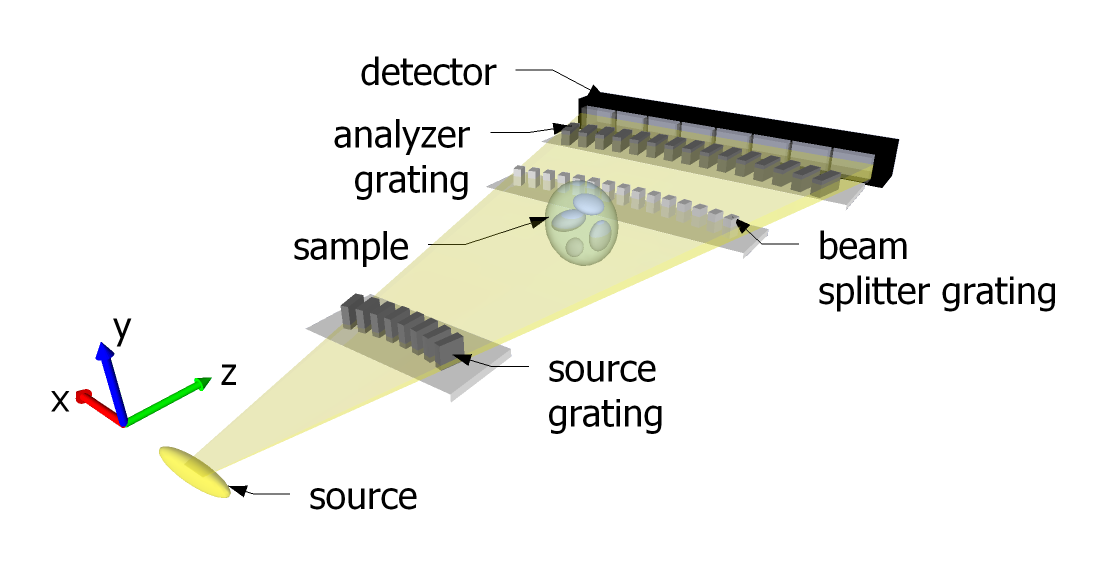
\includegraphics[width=0.6\linewidth]{hDPC_setup.png}
    \captionof{figure}{schematic of the grating interferometer with edge-on
    illumination. The grating structures are circularly aligned in order to
match the fan beam.}
\end{spacedcenter}
In the edge-on configuration, the object is scanned along the vertical
$y$ direction as one line at a time can be acquired.  

%------------------------------------------------

\section*{Grating design}

The gratings were manufactured by Microworks GmbH, Germany, using a LIGA
process. The absorption gratings have a thickness of \SI{800}{\micro\metre}.
All gratings have a pitch $p$ of \SI{2.8}{\micro\metre}.
The interferometers are operated at the first Lohmann distance $d = p / 8
\lambda$.
\begin{spacedcenter}
\begin{tabular}{lll}
    \textbf{design energy} & \SI{100}{\kilo\eV} & \SI{120}{\kilo\eV}\\
    \textbf{intergrating distance} & \SI{15.8}{\centi\metre} &
    \SI{18.9}{\centi\metre}\\
    \textbf{total length} & \SI{54}{\centi\metre} & \SI{61}{\centi\metre}\\
    \textbf{beam splitter} & gold & nickel \\
\end{tabular}
\end{spacedcenter}
\begin{center}
    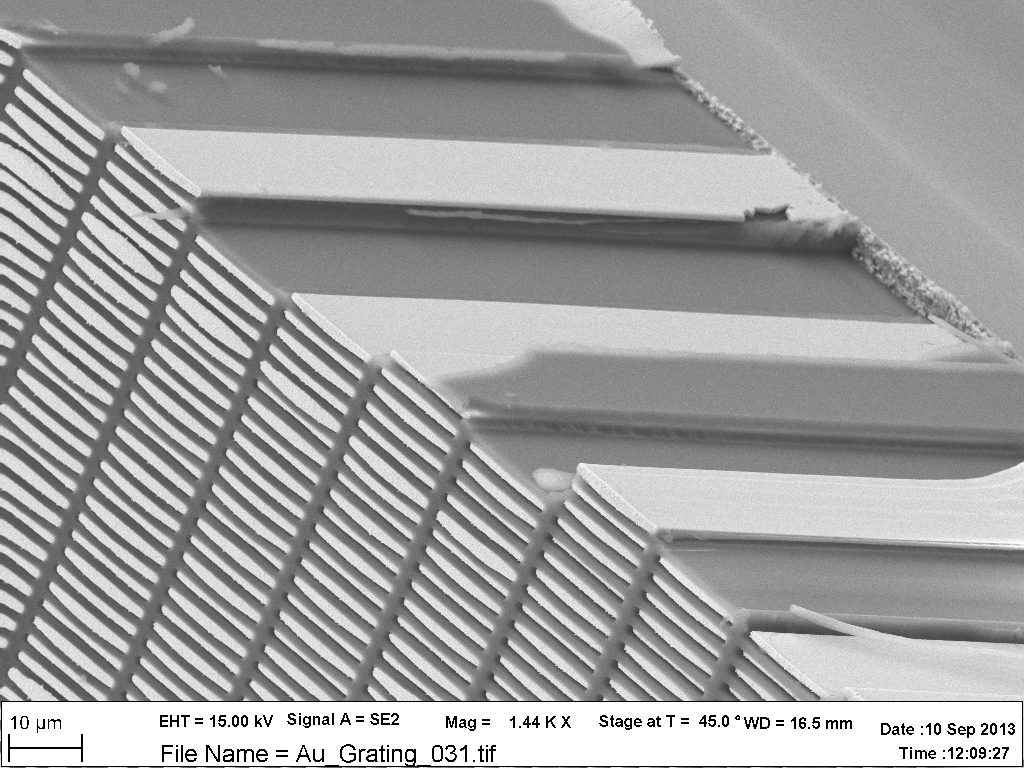
\includegraphics[width=0.5\linewidth]{Au_Grating_031.pdf}
    \captionof{figure}{scanning electron microscope image of the grating structures.}
\end{center}
%\columnbreak


%----------------------------------------------------------------------------------------
%	RESULTS 
%----------------------------------------------------------------------------------------

\section*{Results}
The setups have a rather low average
visibility ($\sim\SI{6}{\percent}$) caused by the low quality of the
gratings. The first images show the three complementary contrasts retrieved
from the phase-stepping procedure \cite{Weitkamp2005}. 
\begin{spacedcenter}
    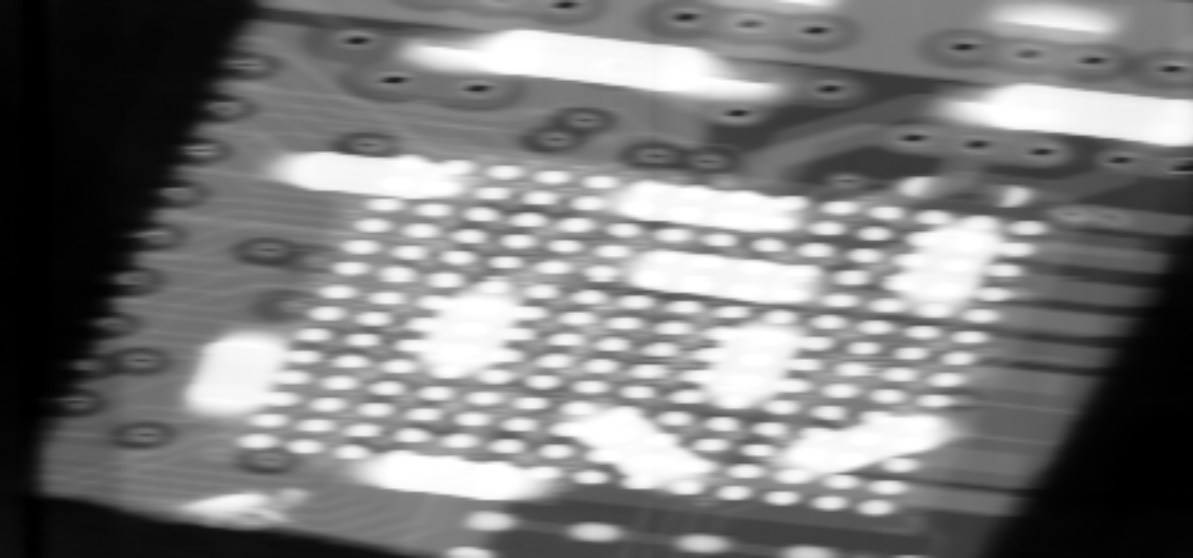
\includegraphics[width=0.3\linewidth,height=8cm]{images_S00075_S00071-img0.png}
    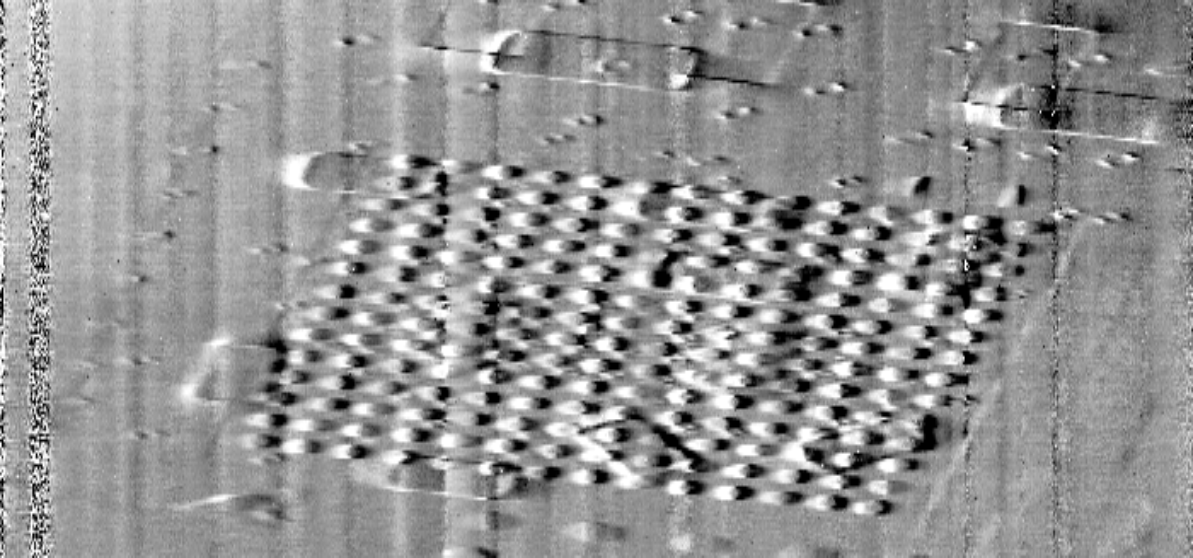
\includegraphics[width=0.3\linewidth,height=8cm]{images_S00075_S00071-img1.png}
    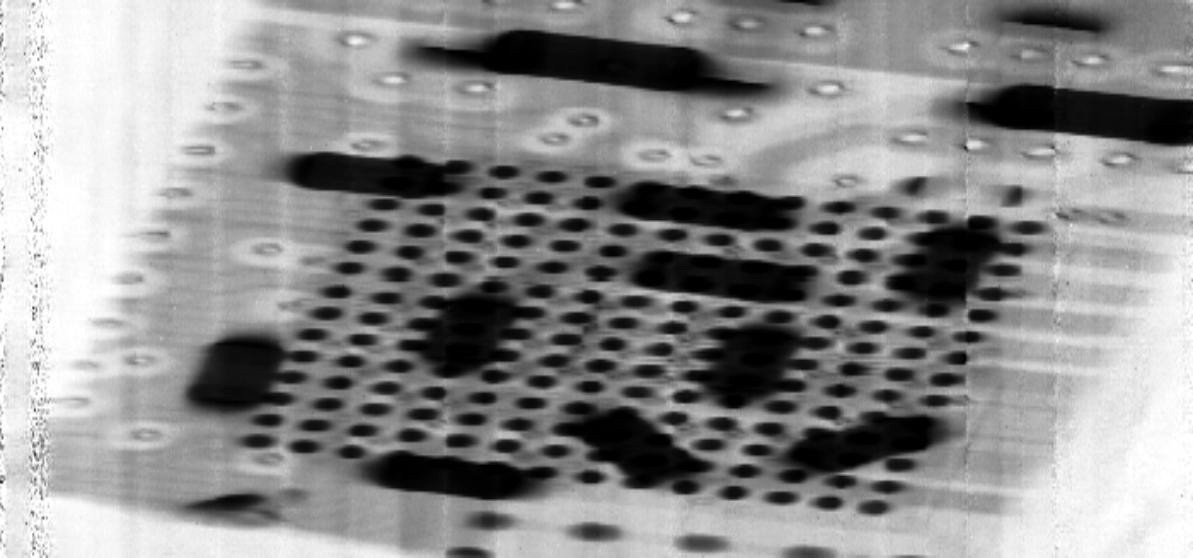
\includegraphics[width=0.3\linewidth,height=8cm]{images_S00075_S00071-img2.png}
    \captionof{figure}{Absorption, differential phase and dark-field image
        of a metal chip scanned in \SI{100}{\micro\m} steps. Field of view
        $\SI{2}{\centi\metre}\times\SI{2}{\centi\metre}$. \SI{100}{\kilo\eV}
    setup.}
\end{spacedcenter}
The exposure time has to be very long (\num{24} phase steps $\times$
\SI{15}{\second} per line) in order to reduce the noise given by the low visibility.
\begin{spacedcenter}
    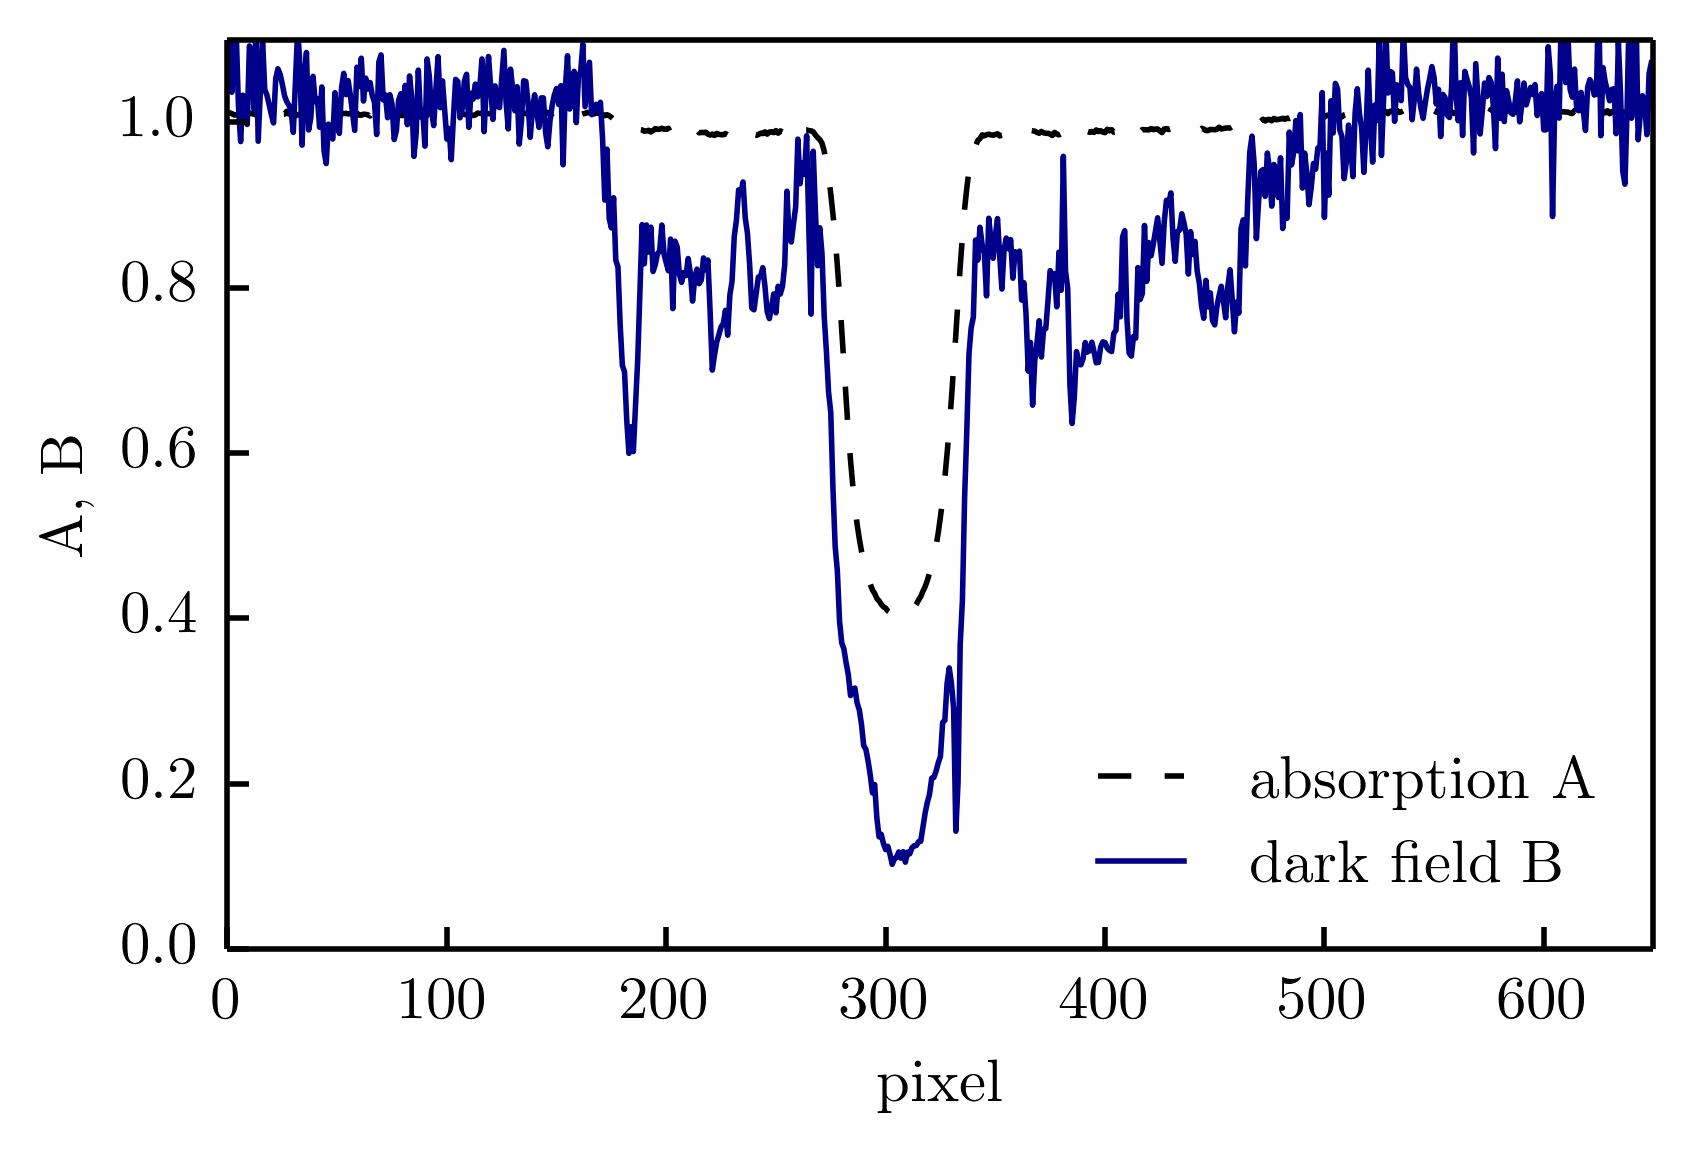
\includegraphics[width=0.6\linewidth]{profile_S00613.png}
    \captionof{figure}{Comparison between absorption and dark field of a
        polystyrene foam with a steel rod with the \SI{120}{\kilo\eV} setup.
        The dark-field contrast is about \SI{20}{\percent} while the soft
        material only absorbs about \SI{2}{\percent} of the radiation.}
\end{spacedcenter}
\color{Navy} 

\section*{Outlook}
\begin{itemize}
    \item This setup demonstrates the feasibility of grating interferometry
        and the availability of the three complementary contrast mechanisms
        at high energies and compact setups.
    \item The technique is very promising for applications on
        conventional sources in the diagnostic energy range between
        \SI{80}{\kilo\eV} and \SI{150}{\kilo\eV}, relevant for material
        science and medical imaging.
    \item Improvements in the fabrication of the gratings will substantially
        decrease the exposure time as the visibility increases.
\end{itemize}

\color{DarkSlateGray} % Set the color back to DarkSlateGray for the rest of the content
 %----------------------------------------------------------------------------------------
%	REFERENCES
%----------------------------------------------------------------------------------------

\bibliographystyle{ieeetr} % Plain referencing style
\bibliography{library} % Use the example bibliography file sample.bib

%----------------------------------------------------------------------------------------
%	ACKNOWLEDGEMENTS
%----------------------------------------------------------------------------------------
\section*{Acknowledgements}

We thank Gordan Mikuljan and István Mohácsi from PSI for the
work on the mechanical design and the SEM images
respectively, Joachim Schulz and Marco Walter from
Microworks GmbH, Germany, for the competent support on grating design
issues, Christian Kottler and Vincent Revol from Centre Suisse
d'Electronique et de Microtechnique (CSEM), Switzerland for the fruitful
discussions on the design of the system. This work has been partially
supported by the Competence Centre for Materials Science and Technology
(CCMX) of the ETH-Board, Project Nr. 61 and by the ERC Grant ERC-2012-StG 310005-PhaseX.
%----------------------------------------------------------------------------------------
\end{multicols}
\end{document}
